\documentclass[11pt]{report}
% PACKAGES
  \usepackage[a4paper,left=28mm,right=28mm,top=30mm,bottom=30mm]{geometry}
  \usepackage{graphicx,epstopdf}      % Used to import external graphics (figures)
  \usepackage{hyperref}       % Used for referring to links inside and outside the document
  \usepackage[table]{xcolor}  % To include colors 
  \usepackage{amsmath}        % For most of the math symbols and environments (such as \begin{align})
  \usepackage{amssymb}        % For using symbols in the document
  \usepackage{float}          % Arranging of figures on the page
  \usepackage[bf]{caption}    % Arranging the captions in floating environments [bf] makes the Figures bold
  \usepackage{subcaption}     % To arrange captions of subfigures
  \usepackage{booktabs}       % For standard tabular tables, with rules
  \usepackage{tabularx}       % For clean tables such as in the Nomenclature
  \usepackage{fancyhdr}       % Fancy headers
  \usepackage[colorinlistoftodos]{todonotes}      % To create todo notes
  \usepackage[nottoc,notlot,notlof]{tocbibind}    % Add bibliography to content
  \usepackage{bm}             % Make bold symbols
  \usepackage{lipsum}
  \usepackage{parskip}
  \usepackage[export]{adjustbox}
  \usepackage{changepage}
% LAY-OUT
  % \usepackage{pdfpages}

  % \usepackage{pdflscape}

   \renewcommand\thesection{\arabic{section}}

  % \usepackage[mathletters]{ucs}
  % \usepackage[utf8x]{inputenc}
  %Bibliography for references, with reference style options
  \usepackage[
  backend=biber,
  bibstyle=ieee,
  citestyle=numeric-comp,
  dashed=false,
  url = false,
  maxnames=8,
  maxcitenames=2,
  mincitenames=1,
  sorting=none,
  isbn = false,
  doi = false
  ]{biblatex}
  \addbibresource{references.bib}

  %Set the page style
  \pagestyle{fancy}
  \fancyhead[L]{\ifodd\value{page} \slshape\nouppercase{\rightmark} \else \fi}
  \fancyhead[R]{\ifodd\value{page} \else \slshape\nouppercase{\leftmark} \fi}
  \chead{ }
  \lfoot{}
  \rfoot{}
  \cfoot{\small\thepage}


  %Give colors to links/refs etc
  \hypersetup{colorlinks, linkcolor={blue!0!black}, 
                          citecolor={blue!70!black}, 
                           urlcolor={blue!80!}} 
                       
  %% Set up numbering and spacing
  \numberwithin{equation}{section}        %Number the equations per section
  \numberwithin{figure}{section}          %Number the figures per section
  \numberwithin{table}{section}           %Number the tables per section
  \captionsetup[table]{skip=1pt}          %Skip 1 pt after a table
  \captionsetup[figure]{skip=3.5pt}       %Skip 4 pt after a figure
  \setcounter{secnumdepth}{3}             %Count up to the subsubsection 
  \setcounter{topnumber}{1}               %Number of floats at top of a page (default is 2)

  %%%%% proof/theorem/definition boxes

  \usepackage{cleveref}
  \usepackage[most]{tcolorbox}
  \newtcbtheorem{Theorem}{Theorem}{
    enhanced,
    sharp corners,
    attach boxed title to top left={
      yshifttext=-1mm
    },
    colback=white,
    colframe=blue!75!black,
    fonttitle=\bfseries,
    boxed title style={
      sharp corners,
      size=small,
      colback=blue!75!black,
      colframe=blue!75!black,
    } 
  }{thm}

  \newtcbtheorem{Definition}{Definition}{
    enhanced,
    sharp corners,
    attach boxed title to top left={
      yshifttext=-1mm
    },
    colback=white,
    colframe=blue!25,
    fonttitle=\bfseries,
    coltitle=black,
    boxed title style={
      sharp corners,
      size=small,
      colback=blue!25,
      colframe=blue!25,
    } 
  }{def}

  \newtcbtheorem[no counter]{Proof}{Proof}{
    enhanced,
    sharp corners,
    attach boxed title to top left={
      yshifttext=-1mm
    },
    colback=white,
    colframe=blue!25,
    fonttitle=\bfseries,
    coltitle=black,
    boxed title style={
      sharp corners,
      size=small,
      colback=blue!25,
      colframe=blue!25,
    } 
  }{prf}
% DEFINITIONS
  %% Titlepage definitions
  \newcommand{\deltitle}{Impact-Aware Control for a Dual-Arm Setup}      %Your project title
  \newcommand{\StudentName}{Gijs van den Brandt}  %Student name
  \newcommand{\StudentID}{1257110}                    %Your student number
  % \newcommand{\DCcode}{2021.109}                      %Get your DC code from the D&C secretariat

  %% Operators
  \DeclareMathOperator\sign{sgn}                      %Sign function
  \DeclareMathOperator\diag{diag}                     %Diagonal operator
  \DeclareMathOperator\imag{Imag}                     %Imaginary part of complex variable
  \DeclareMathOperator\real{Real}                     %Real part of complex variable
  \DeclareMathOperator*{\argmin}{\arg\!\min}          %Argmin operator
  \newcommand{\norm}[1]{\left\lVert#1\right\rVert}    %Norm operator

  %% Variable definition
  \newcommand{\R}{\mathbb{R}}                         % Set of real numbers
  \newcommand{\C}{\mathbb{C}}                         % Set of complex numbers

\begin{document}

% Summary 
  \section*{Progress meeting 11 | 4 November, 2022}


  \section*{1. Progress}
  Parts in red have been added since the previous progress report.
  \begin{itemize}
  
  \item \textbf{Impact detection:} Previously I mentioned that force-based impact detection had some flaws with false positives, and that I wanted to implement position-based impact detection with jump aware filtering as was described by Mark Rijnen. It turns out that this approach also has some limitations. Since the approach is model free, it not possible to tell accelerations caused by impact apart from accelerations driven by the controller in free motion. This becomes a problem for my situation where the impacts have lower accelerations due to the soft covered end effector, and the controller gives high accelerations to track the VR device's velocity reference.

  I realized that impacts cannot be detected from only force or only position estimations. In Section \ref{sec:impact}, I define conditions for an impact, and based on this I propose an impact detection scheme that uses both position and force. This new impact detector has some specific weaknesses that I explain, but so far this impact detector has worked perfectly for my applications with no false positives. I believe I can finally check impact detection off my todo list.

  \item \textbf{Reference spreading with impedance control:} With impact detection, I could finally implement reference spreading on the setup. I performed a stamping experiment similar to Sven, where the end effector moves downward and collides with a fixed surface. In varying experiments, the fixed surface was lowered by 10mm or raised by 30mm, and the tests were ran with- and without reference spreading. The results are shown in Section \ref{sec:RS}.

  It turns out that reference spreading does not provide any significant value to impedance control. The reference extracted from the VR device does not contain jumps, meaning that RS does not provide the benefit of aligning the jumps in the reference with detected impacts to prevent error peaking. Nevertheless, the tracking error still contains a jump. An impact map could be used to match the post-impact velocity reference to the post-impact velocity of the system. Initially I envisioned that an impact map would not be necessary since the velocity jump could be estimated from the demonstration, however the current implementation only looks at the VR device. Some decisions must be made here since RS currently has no value, and without out it, the controller cannot be considered impact-aware.

   \textcolor{red}{Evaluating reference spreading is one of the key goals of my project, and to do that, the velocity reference must contain jumps. Therefore I implemented a controller that tracks the position/velocity of the robot arm during demonstration (so not the VR device). I used feed forward to control the contact force, which worked as desired in simulation. Experiments on the real system were less succesful, presumably due to friction, though this still needs more investigation. Nevertheless, I will discuss with Jari if feedforward really is the way to go.  }

  \item \textbf{Teleoperation:} Last time, I mentioned that a velocity reference results in more responsive tracking of the VR device. This was paired with the safety limits of the robot being exceeded in edge cases (mostly with fast rotations). As a solution, I looked into the task weights, however these weights only make a difference by prioritizing certain tasks when not all tasks can be executed perfectly. This was not the problem however; even when the impedance task can be executed perfectly, rotational errors cause the controller to apply a virtual torque, which often is paired with the fast translational displacements. Instead of altering weights, I solved the problem by limiting the velocity reference to 1 m/s or 0.7 rad/s. An alternative approachis to use a force sensor to decouple translational and rotational impedance DoF's, though I decided that further investigation of this was not a priority.

   \textcolor{red}{Alessandro suggest that I move the point on the robot that I try to control to be in line with the wrist joints of the robot. This allowed for better tracking of the angular DoF's without exceeding safety constraints. Furthermore, I removed the velocity limit that I previously applied to the VR device signals, and am now limiting the impedance wrench instead. I can now reach end effector velocities of 1.5 m/s and 1.5 rad/s.}

  Furthermore I added a feature where the VR device vibrates to indicate how much force is detected at the end effector. Personally I had difficulty with correlating the vibration with a force when teleoperating, and it also appeared that the vibrations were affecting the velocity reference extracted from the VR device. Overall I prefer teleoperation without the vibration.
    \color{red}
  \item  \textbf{Misc:}  I made a pallet of 40x60 cm for making nicer videos/demos. Furthermore I started on the introduction of my final report. I also looked into some questions Alesandro had about Sven's work:

  \textbf{Did Sven use the VR device or a hardcoded reference for the demonstrations?}
  Sven ended up using hardcoded references (with small randomly generated variances) to ensure that the impact occurred under relatively similar conditions

\textbf{Did Sven use the same impedance controller used during demonstration and replays?}
  Yes, the controller used during demonstration is the same as the ante-impact phase controller. The stiffnesses also remain unchanged (400 N/m in x and y direction, 1080 N/m in z direction, and 50 Nm/rad in orientation. For comparison, I am using 800 N/m and 50 Nm/rad) 

\textbf{Did Sven apply reference spreading to the VR device position or to measured robot positions/velocities/forces during the demonstration?}
  Reference spreading was applied to robot measurements during the demonstration. 
\color{black}
  \end{itemize}

  \section*{2. Agenda}
  During the meeting, I would like to discuss the following points:

  \begin{itemize}
      \item During the last meeting, we did not have the time to talk about impact discussion, so let's go over that today.
      \item Previously, it was proposed that I should write a paper+appendix rather than a report. Is this decision final? And are there any guidelines you recommend for writing such a paper?
      \item For the contact phase controller, I want to discuss with Jari, but if time allows it we can already talk about it during this meeting.
  \end{itemize}

  \section*{3. Next steps}

  \begin{itemize}
      \item Implement a contact-phase controller that does not need a complete model of the environment (for example, I do not know the location of the box).
      \item Compare the performance of the controller with and without reference spreading
      \item Reporting
  \end{itemize}

  \section*{4. Long-term planning}
  Shown below is the current long-term planning for the project phase.  I believe that impact detection is finally finished. I have added another two weeks to the RS controller, but further extensions would start to interfere with writing my report.

  \begin{figure}[H]
  \centering
  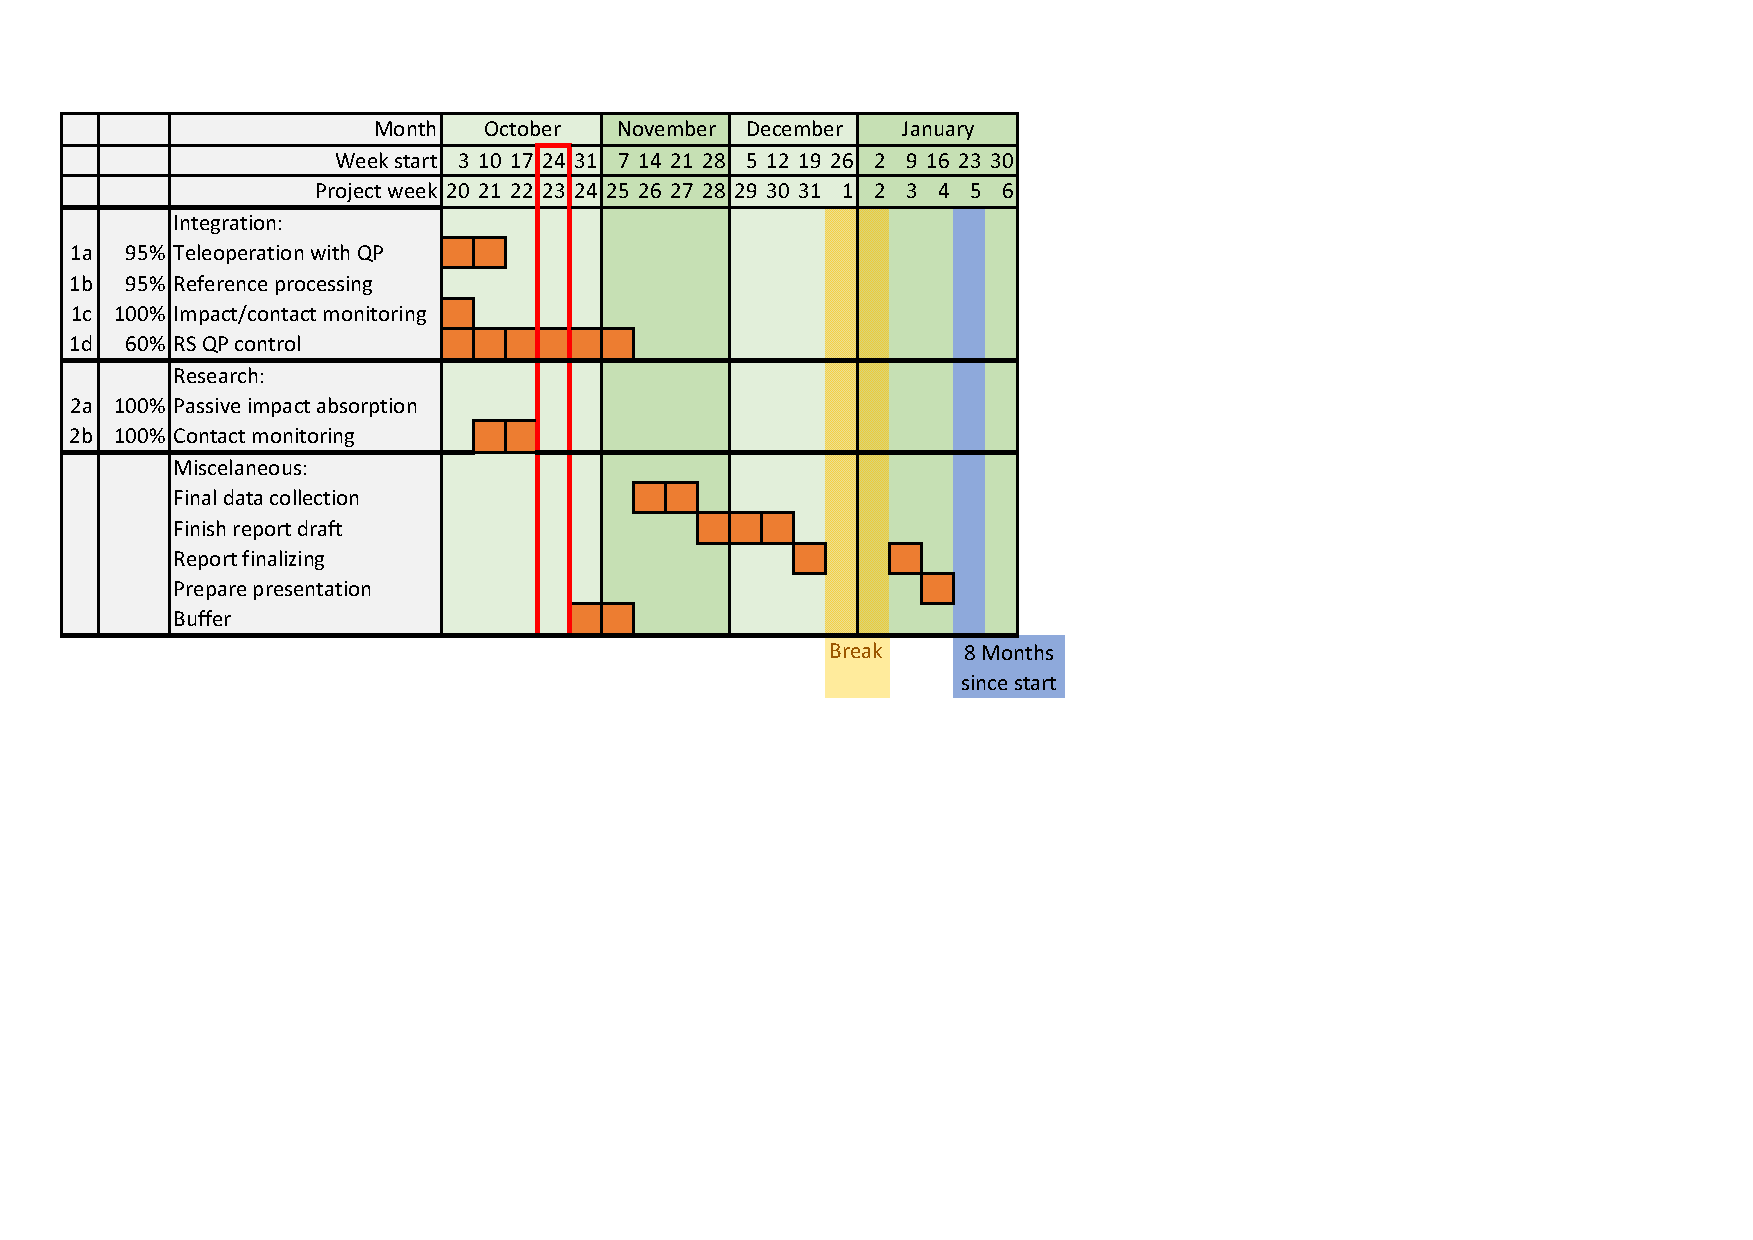
\includegraphics[width=0.7\textwidth, trim={0.87cm 9.5cm 10cm 1.5cm},clip]{Graphics/planning v2.pdf}

  \label{fig:my_label}
  \end{figure}

  \begin{enumerate}
  \item[1a] \textbf{Translating dual-arm teleoperation to the physical setup.} The existing implementation in simulation already uses the mc\_rtc interface, meaning that the switch to reality shouldn't pose an issue. Nevertheless, this step also involves getting familiar with the software, which increases the anticipated time for this step.
  \item[1b] \textbf{Extracting references from the demonstration data.} The demonstrated trajectories should be split into ante-impact and post-impact sections, and extended to facilitate RS. Furthermore multiple measurements should be used to fit ProMPs, after which a reference can be generated. It is also key to identify which data should be learned from the demonstration. This is not limited to choosing between a force or position reference, but can also consists of learning properties of the environment, e.g. friction cones or box inertia, that are crucial to a dual-arm box grabbing scenario.
  \item[1c] \textbf{Integrating impact detection and contact monitoring in mc\_rtc.} The majority of the impact detector's complexity resides in the momentum observer; however, Franka Emika's software already has an integrated momentum observer. This still leaves tuning of the impact detecting algorithms which might be time consuming. Furthermore an analysis comparing the available methods could be worthwhile. Factors which determines the effectivity of the impact detection algorithm include speed of detection, as well as reliability, i.e. the rate of false positives. The addition of objects that cause unexpected impacts is not considered a part of the research scope.
  \item[1d] \textbf{Configuring QP controllers for the ante-impact, intermediate, and post-impact phase.} For each of the phases, it is important to address the redundancy in the arms' degrees of freedom. After that, control for the ante-impact phase should be trivial. For the intermediate phase, it is expected that ante-impact reference tracking without velocity feedback should be applicable on a dual-arm robot, though this might prove to be false, in which case other methods should be investigated. During post-impact control, the challenge will be maintaining non-slip contact with the box. It is difficult to say how well the results from simulations can be repeated with torque control, where the state of the box can not be sensed to be used in the QP controller.
   \item[2a] \textbf{Passive impact absorption:} A soft cover for the end effector will be designed. Such a cover can be connected to the Panda by connecting bolts to the so-called flange interface. A mold will be created using 3D printing to allow for casting of various silicone soft covers. Design parameters -- i.e. material properties (controlled by choosing different kinds of silicone) and soft cover thickness -- will be analyzed experimentally. A systematic comparison between various designs will require an experiment plan including a realistic testing scenario. Evaluation of performance can be based on the oscillatory response in position and force after establishing contact. Furthermore multiple scenarios with various box surface properties and robot poses should be considered.
  
  \item[2b] \textbf{Contact monitoring:} When investigating contact monitoring, two approaches can be taken: either using proprioceptive or exteroceptive sensors. A possible improvement for contact monitoring using proprioceptive sensors could be to wait a fixed time starting from the last detected impact, rather than waiting a fixed time from the first impact. As for exteroceptive sensors, they can be a hurdle for large-scale commercial applications as they are not integrated in the robot. However, if a soft cover is to be mounted to the end effector, including tactile sensors for impact and contact monitoring becomes more feasible. Practical questions such as which tactile sensor to use and how to integrate it could be addressed, though this is not absolutely necessary for completing the research goals, and therefore has a low priority.
  \end{enumerate}
% main text
  \newpage
  \section{Impact detection}\label{sec:impact}
  I performed an experiment with position-based impact detection as described by Mark Rijnen, and force-based impact detection as was implemented by Benn Proper. Firstly I will give a brief explanation of how these schemes work.

  \subsection{Position-based impact detection}
  This scheme is model free: it only requires position measurements $q_k$ where $k$ indicates the timestep. A polynomial of degree $K$ is fitted to the previous $M+1$ measured positions contained in $\bar{q}_k = \begin{bmatrix} q_{k-M}& ... & q_{k} \end{bmatrix}$. This polynomial can be used to find a predicted position $\tilde{q}_k$ during a future time $t_{k+1}$, i.e., $\tilde{q}_{k+1}=P(t_{k+1},\bar{q}_k)$. A large prediction error $e_{k}=\left \|  \tilde{q}_{k}-q_{k}\right \|$ can be the result of a large acceleration, possibly caused by an impact. An impact is detected when the error $e_k$ exceeds a bound.

  \subsection{Force-based impact detection}
  For this method, external force estimate $\tilde{F}_k$ derived using a momentum observer. A force-rate $\dot{\tilde{F}}$ is determined following $\dot{\tilde{F_k}}=\frac{\tilde{F_k}-\tilde{F}_{k-1}}{t_k-t_{k-1}}$. If the absolute value of this force-rate exceeds a bound, an impact is detected.

  \subsection{Evaluation}
  Figure \ref{fig:force_pos_detection} shows the results of an experiment where both impact detection schemes were applied. The end effector moves downward and impacts table, after which the end effector is lifted and then moved downward for a second impact. For the position-based impact detector, window length $M=10$ and polynomial order $K=2$ were used. 

  The position-based impact detector error $e$ shows peaks while in free motion. These peaks are more prominent than the peak that happens right before the moment of impact. This is a result of aggresive tracking of the VR device and small acceleration during impacts due to the soft end effector. No bound can be defined so that impacts can be isolated, meaning that this approach is not useful for the scenario.

  The force-based impact detector does not suffer from large peaks during free motion. Still, a peak can be seen at $t=14$ s where contact is lost. Similiar peaks will appear when the force is increased over a short time, despite there being no loss of contacts. No bound can be chosen so that the true impacts are isolated from the other events with high force rates.

  Conclusively, neither the force nor the position-based impact detector is useful for this situation. This motivates the development of a new method in the next section.

  \begin{figure}[]
  \centering
  \begin{adjustwidth}{0pt}{5pt}
  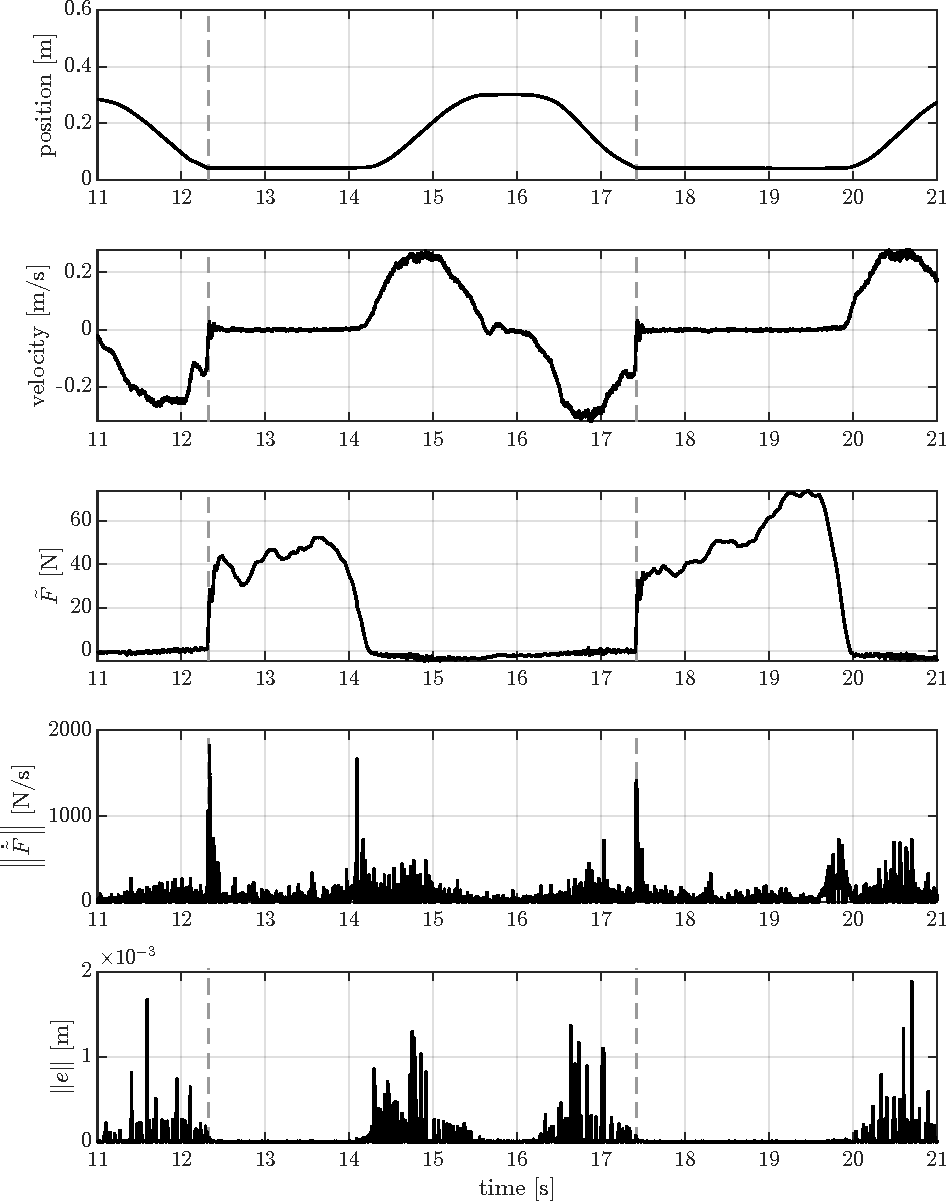
\includegraphics[right]{Graphics/force_VS_pos_impacts.pdf}
  \end{adjustwidth}
  \caption{Result of an experiment featuring two impacts. Only results in downward direction are shown. The vertical dashed lines are detected with a newly-proposed method.}
  \label{fig:force_pos_detection}
  \end{figure}
\newpage
  \subsection{Hybrid impact detection}
  Relatively large accelerations and force rates may be caused by impacts, though they are not sufficient conditions. To formulate an alternative impact detection scheme, firstly an impact is formally defined.

  Let there be two bodies named A and B, see Figure \ref{fig:bodies}. The relative velocity of body A with respect to B is $\vec{v}_{A,B}$. Furthermore, when in contact, the bodies exert a force $\vec{F}$ on each other. We can say that an impact has occurred between time-steps $t_1$ and $t_2$, with $t_2>t_1$, if the following sufficient conditions are met:
\begin{enumerate}
  \item $\left \| \vec{F}_{t_1} \right \|= 0$
  \item $\left \| \vec{F}_{t_2} \right \|> 0$
  \item $(\vec{v}_{A,B})_{t_1} \cdot \vec{F}_{t_2} < 0$.  
  % \item $\frac{\vec{v}_{t_1}\dot$\vec{F}_{t_2}}{ \left \| \vec{F}_{t_2} \right \| }  > 0$
\end{enumerate}
  
 \begin{figure}[]
  \centering
  % \begin{adjustwidth}{0pt}{5pt}
  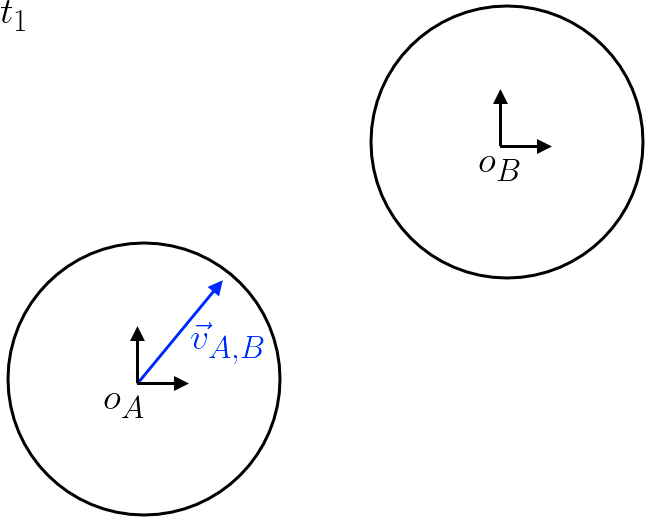
\includegraphics[width=0.4\textwidth]{Graphics/1.png}\hfill
  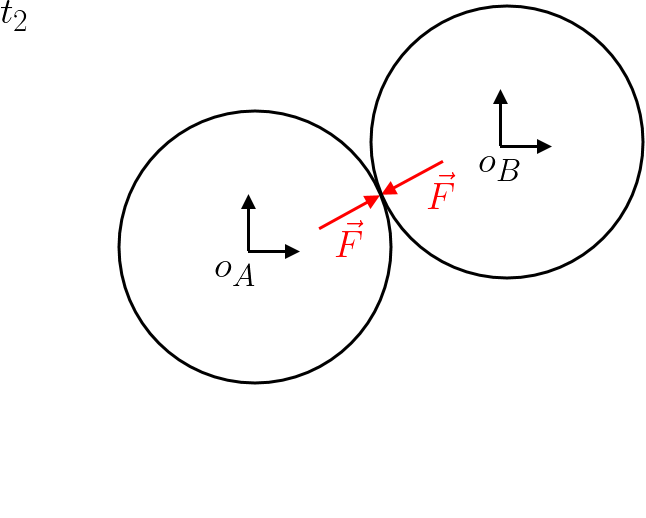
\includegraphics[width=0.4\textwidth]{Graphics/2.png}
  % \includegraphics[right]{Graphics/result_torque0mm.pdf}
  % \end{adjustwidth}
  \caption{Two bodies before and after impact}
  \label{fig:bodies}
  \end{figure}

  The third conditions evaluates the velocity in direction of the force vector to ensure that contact was not already previously established. Without it, an impact may be detected between two bodies that do not move.

  In practice, these conditions are hard to evaluate. We do not know the velocity of the end-effector to the contact surface, and the force estimations are hardly ever exactly equal to zero. Therefore, the conditions are changed to

  \begin{enumerate}
  \item $\left \| \vec{F}_{t_1} \right \|< b_F$
  \item $\left \| \vec{F}_{t_2} \right \|> 2b_F$
  \item $(\vec{v}_{E,W})_{t_1} \cdot \vec{F}_{t_2} < -b_v$  
\end{enumerate}
  where $b_F$ and $b_v$ are bounds that should be larger than errors in the force and velocity estimations respectively. Furthermore $\vec{v}_{E,W}$ is the velocity of the end effector with respect to the world frame.

  These more practical conditions are not perfect. Low-velocity impacts or impacts with low forces will not be detected. Furthermore, when the robot is static and another object bumps into it, this will not be classified as impact. This method is also limited to one contact at a time, since the momentum observer cannot distinguish between various sources of exteral force. Nevertheless, this is not a problem in the desired usecase, and more importantly, there will be no false-positive impact detections. 

  The hybrid impact detection method was evaluated experimentally. The vertical lines in Figure \ref{fig:force_pos_detection} are the results of this impact detection scheme, with $b_F = 8$ N, and $b_v = 0.05$~m/s. 

  \section{Impedance control with reference spreading}\label{sec:RS}
  To evaluate impedance control with reference spreading, firstly a demonstration was performed where the end effector stamps the table twice. A metal plate with a thickness of approximately 10mm was placed on the table during the demonstration, so that it may later be removed to move the impact surface. The extracted and extended references in z-direction are shown in Figure \ref{fig:spreading}.

  The generated references were applied in configurations where the impact surface was 10 mm lower, the same height, or 30 mm higher. Furthermore each of these configurations was evaluated with- and without reference spreading. The results are shown in Figure \ref{fig:results_-10mm}-\ref{fig:results_30mm}. 

  Looking at the figures, there are no significant improvements when using reference spreading as opposed to not using reference spreading when looking at tracking errors, external forces, or motor torques. Since the reference is based on the motions of the VR device, the reference does not contain any jumps, and therefore reference spreading does add the value of aligning jumps in the reference and in reality. This is visualized in Figure \ref{fig:RSvive}.

  There might still be some opportunities with reference spreading, however this would require a jump to be introduced in the reference. This could be done based on the jumps in the tracked velocity during the demonstration. It should be considered, however, whether introducing jumps into a reference is actually beneficial. Another approach could be briefly reducing damping after impact, or setting the velocity reference to zero for a short while.


\vfill
    \begin{figure}[!h]
  \centering
  \begin{adjustwidth}{0pt}{5pt}
  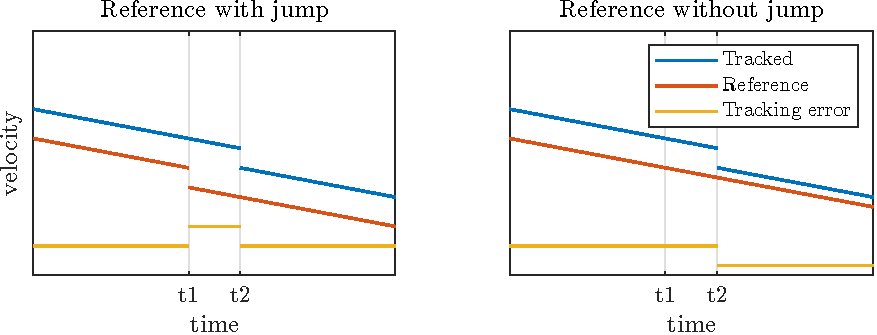
\includegraphics[right]{Graphics/RSvive.pdf}
  \end{adjustwidth}
  \caption{When the reference contains a jump that is misaligned with the jump that is actually tracked, the error peaks. When the reference does not contain a jump, as is the case with the reference directly extracted from the VR device during demonstration, there is no peak in the tracking error.}
  \label{fig:RSvive}
  \end{figure}

  \begin{figure}[]
  \centering
  \begin{adjustwidth}{0pt}{5pt}
  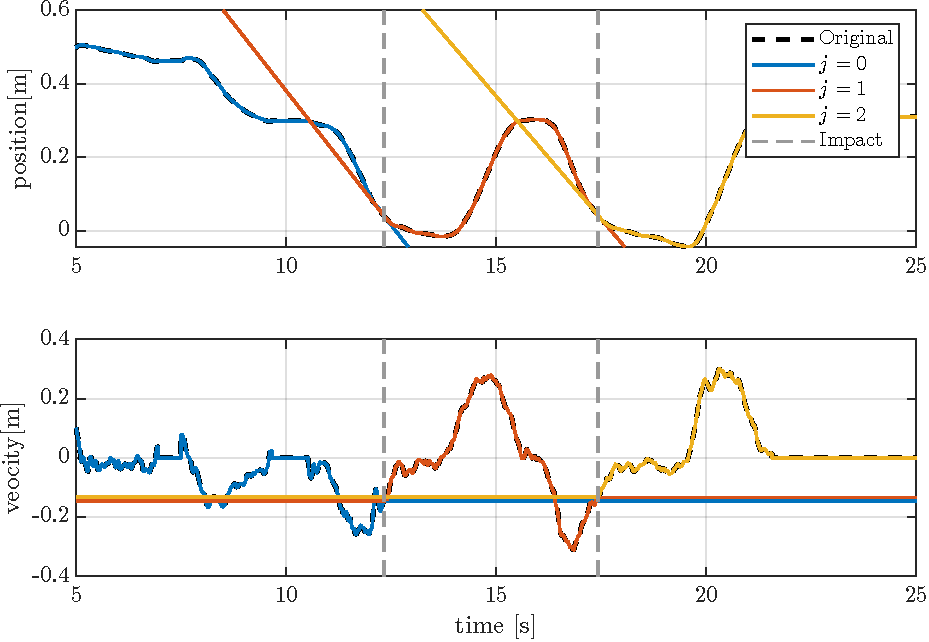
\includegraphics[right]{Graphics/spreading.pdf}
  \end{adjustwidth}
  \caption{Reference extracted for stamping task, together with the extended references. The value of $j$ relates to how many jumps have occurred.}
  \label{fig:spreading}
  \end{figure}

 \begin{figure}[]
  \centering
  \begin{adjustwidth}{0pt}{5pt}
  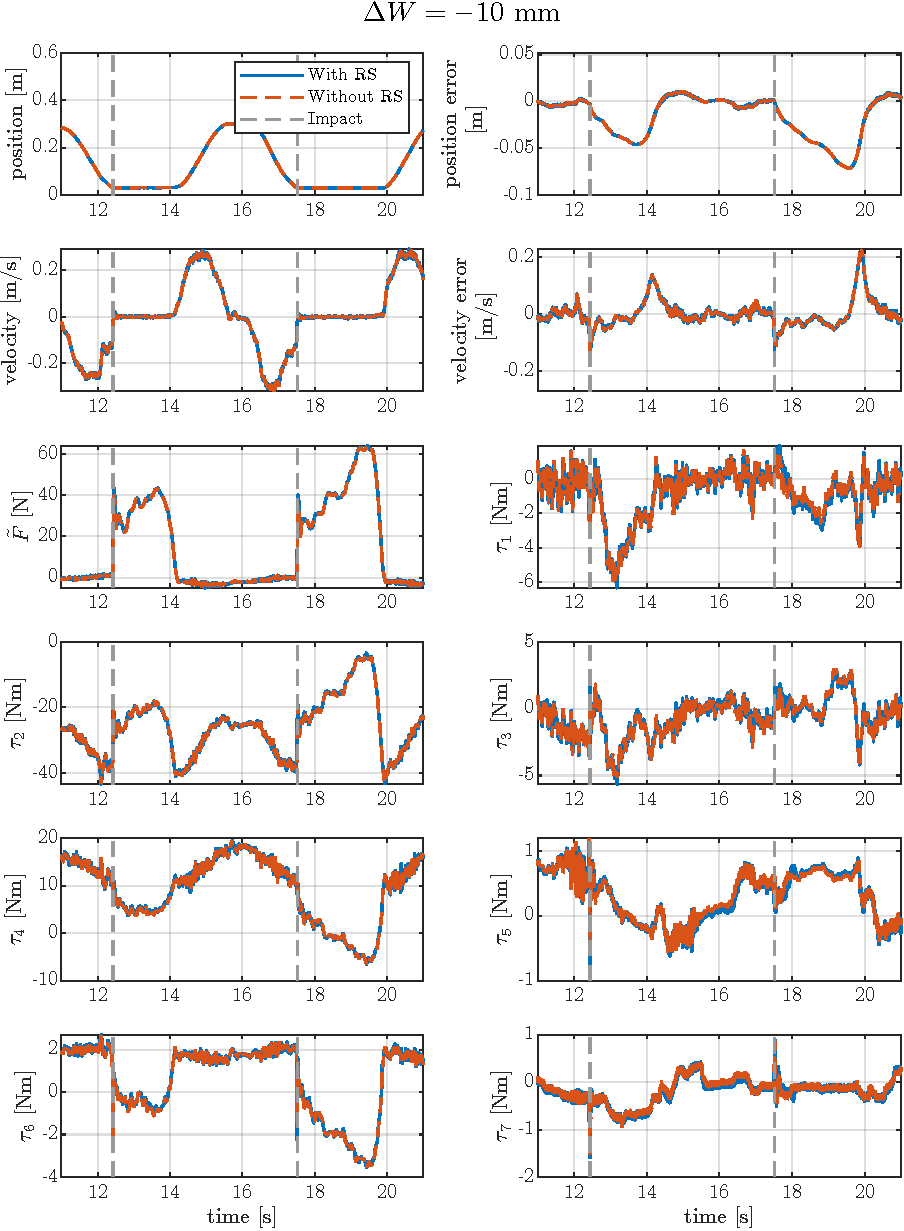
\includegraphics[right]{Graphics/result-10mm.pdf}
  % \includegraphics[right]{Graphics/result_torque-10mm.pdf}
  \end{adjustwidth}
  \caption{Results of stamping experiment with and without reference spreading. Only the z-direction in carthesian space is shown. The contact surface is 10 mm lower than during the demonstration.}
  \label{fig:results_-10mm}
  \end{figure}


 \begin{figure}[]
  \centering
  \begin{adjustwidth}{0pt}{5pt}
  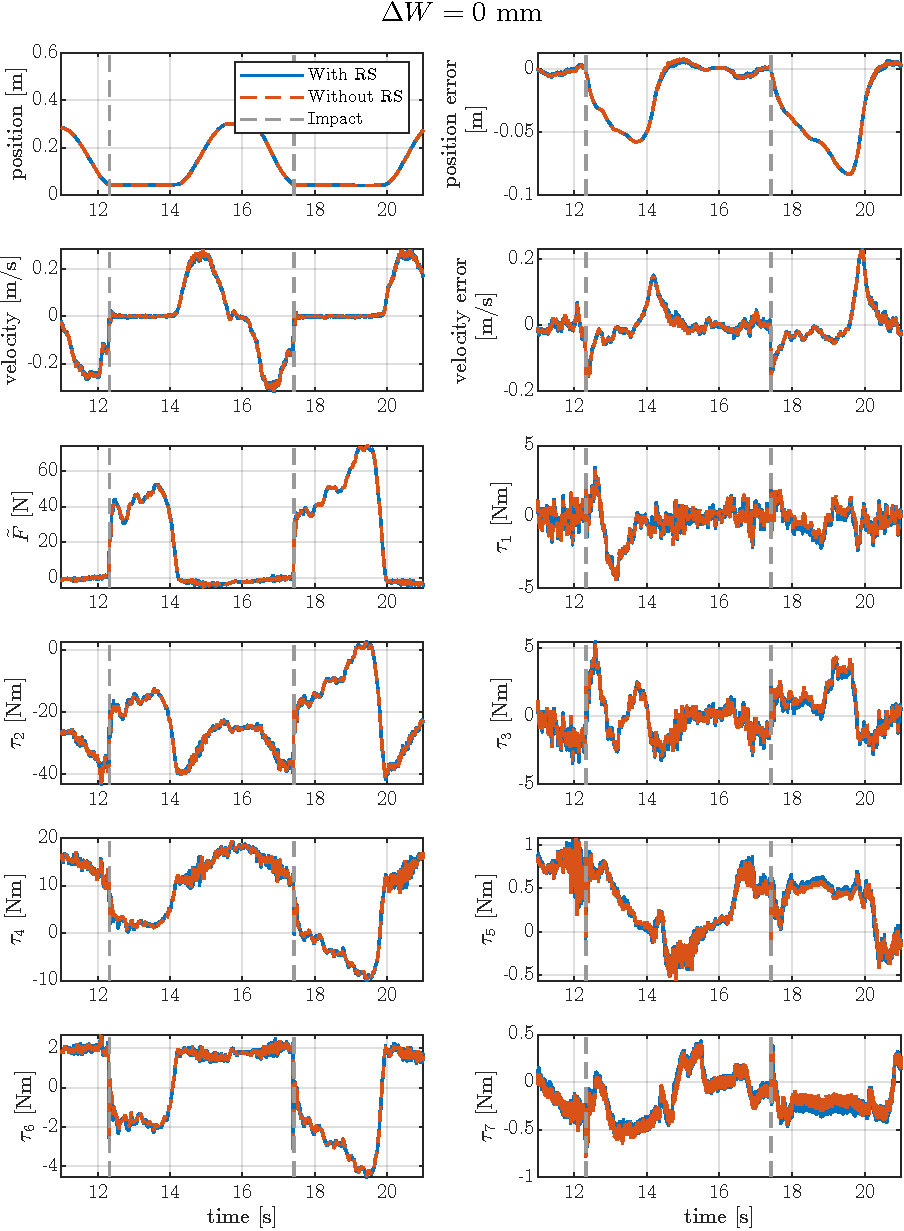
\includegraphics[right]{Graphics/result0mm.pdf}
  % \includegraphics[right]{Graphics/result_torque0mm.pdf}
  \end{adjustwidth}
  \caption{Results of stamping experiment with and without reference spreading. Only the z-direction in carthesian space is shown. The contact surface is the same height as during the demonstration.}
  \label{fig:results_0mm}
  \end{figure}

 \begin{figure}[]
  \centering
  \begin{adjustwidth}{0pt}{5pt}
  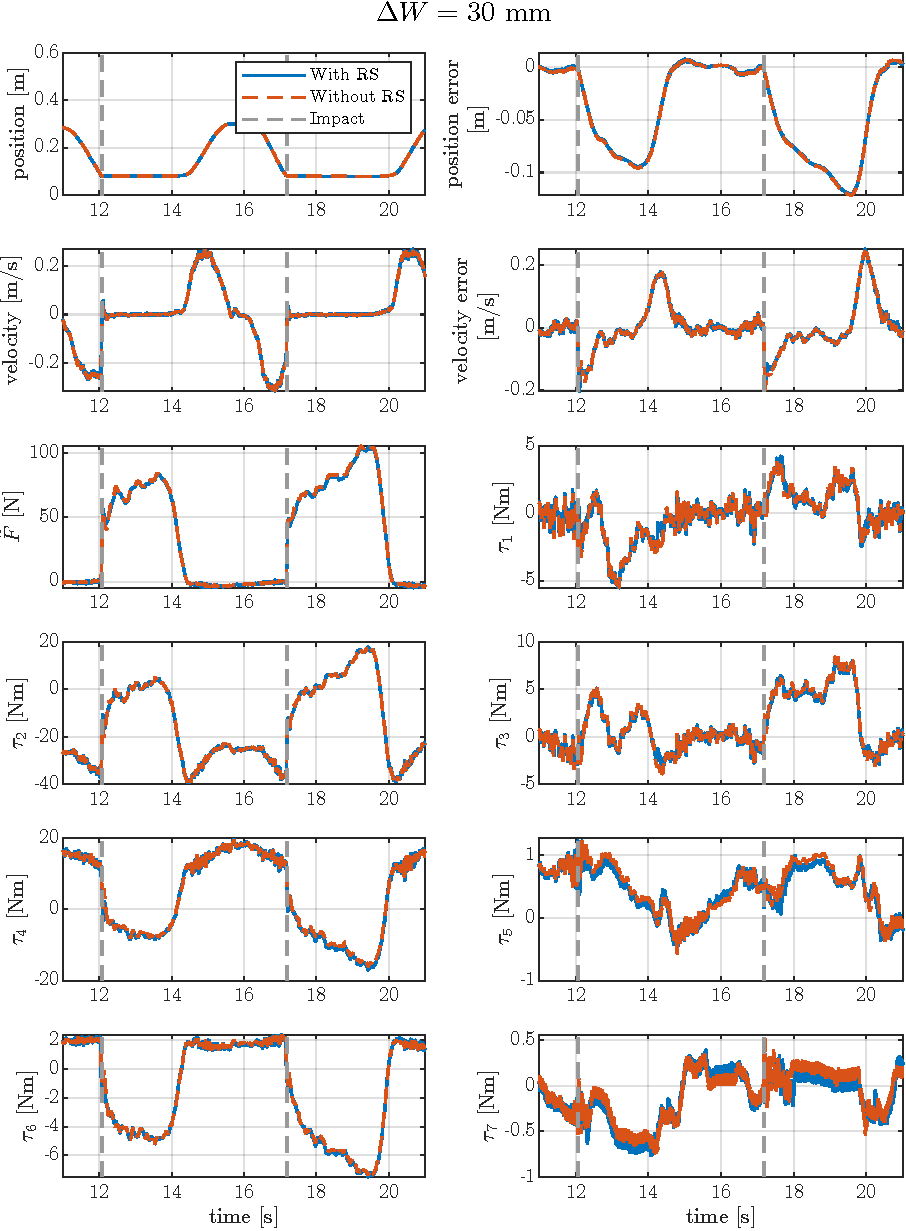
\includegraphics[right]{Graphics/result30mm.pdf}
  % \includegraphics[right]{Graphics/result_torque-10mm.pdf}

  \end{adjustwidth}
  \caption{Results of stamping experiment with and without reference spreading. Only the z-direction in carthesian space is shown. The contact surface is 30 mm higher than during the demonstration.}
  \label{fig:results_30mm}
  \end{figure}
% BIBLIOGRAPHY

  \newpage
  \addcontentsline{toc}{chapter}{References}
  \printbibliography[title=References]

  \newpage
  \thispagestyle{empty} \ \newpage


\end{document}